\section*{6\quad Does a depth advantage persist at scale?}
\topic{E8.} We widened the shared Boolean-program block to 896, 1,600 and 2,880 hidden dimensions. Every parameter belongs to an active computation or readout. The first ladder used 16 updates and 1,024 input token presentations per fit, with three paired seeds for fixed four and adaptive. It was a feasibility test. Training-time profiling motivated a second, separately registered 45-fit ladder with five independently trained models, three sizes and three seeds. Each fit received 160 updates, 1,280 examples and 40,960 input token presentations at length 32. The test used a new 256-example draw. The parameter count and training cost change together across sizes.
\begin{center}\small\begin{tabular}{lrrrrrr}\toprule
Params & MORPH, \% & Fixed 1 & Fixed 2 & Fixed 3 & Fixed 4 & Train TFLOPs\\\midrule
9.65M & 67.19 & 63.54 & 67.71 & 69.40 & 60.42 & 9.53\\
30.76M & 67.19 & 63.28 & 59.64 & 62.89 & 56.64 & 30.30\\
99.60M & 62.37 & 68.10 & 65.23 & 72.01 & 60.42 & 98.03\\
\bottomrule\end{tabular}\end{center}
\captext{Accuracy values are percentages on the controlled synthetic task. The last column is adaptive training arithmetic per fit. At each width the fixed-four model closely matches both the adaptive model's trainable parameters and its training arithmetic. Fixed one through four locate its inference frontier.}
\begin{center}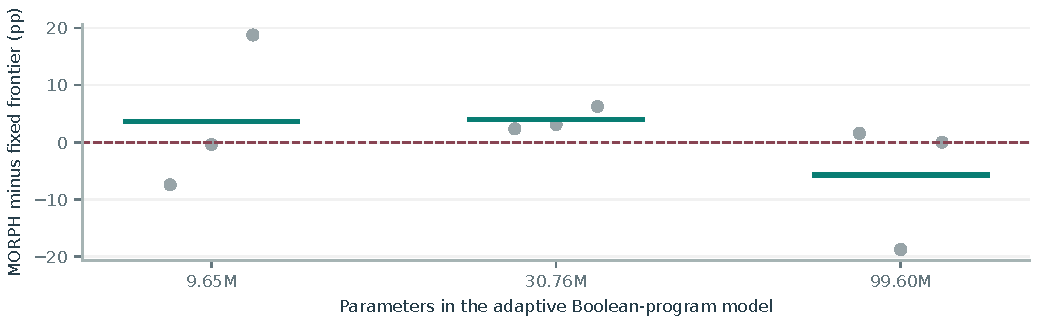
\includegraphics[width=.93\linewidth]{figures/scaling.pdf}\end{center}
\captext{Figure 2. Adaptive accuracy minus the best feasible fixed model or input-independent fixed mixture. Points are paired training seeds. Teal lines indicate means; zero indicates parity.}
\topic{Primary comparison.} The respective gains in percentage points at the three sizes were +3.65 [$-$30.00, +37.29], +3.91 [$-$1.23, +9.04], $-$5.73 [$-$33.81, +22.35]. On the original 16-update ladder adaptive accuracy was 46.88\%, 51.04\%, 50.00\%. Different test drawings and training schedules make the two ladders unsuitable for estimating a causal effect of training duration.
\topic{Calibration sensitivity.} Every scaled adaptive model chose one pass on every test case with the registered threshold grid. The three accuracy differences therefore cannot establish useful input-dependent depth. A post-hoc finer threshold search produced variation. Using only the original stored hazards, we calibrated on the first half of each archived test set and scored the second half. The gains against the fixed frontier at the three sizes were $-6.12$, $-2.97$ and $-7.78$ pp. Because this analysis was designed after the original tests, it is exploratory. Retraining discarded checkpoints changed some original-threshold predictions in five of twelve diagnostic records. The main tables use the original predictions. The companion data distinguish same-weight cached comparisons from retraining.

